\subsection{Controlabilidad y observabilidad de sistemas lineales}

Sea el sistema 
\[(1)
    \left\{
        \begin{array}{lll}
            \dot{x}(t) = \overbrace{ A }^{ \text{estabilidad} }x(t) + \underbrace{ B }_{ \textbf{controlabilidad} }u(t) \\
            y(t) = Cx(t)
        \end{array}
    \right.
\]

donde 
\[
    \begin{split}
        X & : n \times 1 \\
        A & : n \times n \\
        B & : n \times m \;\; entradas \\
        u & : m \times 1 \\
        C & : p \times n \\
        y & : P \times 1 \;\; salidas
    \end{split}
\]

Controlabilidad: existencia de una entrada \( u(t) \) tal que cada variable de estado se pueda manipular de manera independiente, es decir, las entradas cambian las variables.

Observabilidad: Consiste en determinar el estado inicial a partir de la salida \( y(t) \), es decir, las condiciones iniciales afectan la salida.

\begin{figure}[h!]
    \centering
    \begin{subfigure}[b]{0.45\linewidth}
        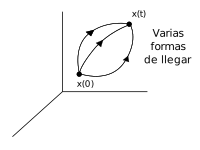
\includegraphics[scale=0.25]{Control de Sistemas Mecatronicos Figuras/01 Controlabilidad}
        \caption{Controlabilidad}
    \end{subfigure}
    \begin{subfigure}[b]{0.45\linewidth}
        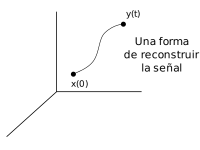
\includegraphics[scale=0.25]{Control de Sistemas Mecatronicos Figuras/02 Observabilidad}
        \caption{Observabilidad}
    \end{subfigure}
\end{figure}

Definición 1. El sistema (1) es controlable si existe \(u(t)\) tal que para todo estado inicial \( x_{0}=x(0) \) y todo estado final \(x_{f}=x(T)\), el sistema puede llevarse de \( x_{0} \) a \( x_{f} \) en tiempo finito.